\begin{problem}{Chia cây}{treecut.inp}{treecut.out}{1 giây}{256 megabytes}
 
 
Bạn có một cây gồm $n$ đỉnh, các đỉnh được đánh số từ $1$ đến $n$. Đỉnh thứ $i$ có giá trị $a_i$. Nhắc lại, cây là một đồ thị vô hướng, liên thông và không có chu trình. 

Bạn có thể tùy ý xóa bớt một số cạnh trên cây (có thể không xóa cạnh nào), khi đó cây sẽ bị chia thành nhiều thành phần liên thông riêng biệt. 

Giá trị của một thành phần liên thông được định nghĩa là hiệu của giá trị lớn nhất của một đỉnh thuộc thành phần liên thông đó và giá trị nhỏ nhất của một đỉnh thuộc thành phần liên thông đó. Nói cách khác, với một thành phần liên thông $S$, giá trị của $S$ là $\max_{u \in S}a_u - \min_{u \in S}a_u$.

Giá trị của một cách xóa cạnh là tổng giá trị của các thành phần liên thông được tạo ra trong cách xóa cạnh đó.

\textbf{Yêu cầu:} Hãy tìm cách xóa cạnh có giá trị lớn nhất.
 
\InputFile
\begin{itemize}
\item Dòng thứ nhất chứa một số nguyên $n$ ($1 \le n \le 3 \cdot 10^5$) là số đỉnh của cây.
\item Dòng thứ hai chứa $n$ số nguyên $a_1, a_2, \dots, a_n$ ($1 \le a_i \le 10^9$) mô tả giá trị của các đỉnh.
\item Dòng thứ $i$ trong $n - 1$ dòng tiếp theo mỗi dòng chứa hai số nguyên $u_i$, $v_i$ ($1 \le u_i, v_i \le n$) mô tả một cạnh trên cây. Dữ liệu đảm bảo các cạnh này tạo thành một cây.
\end{itemize}

Hai số nguyên liên tiếp trên một dòng cách nhau bởi một dấu cách.
 
\OutputFile
In ra một số nguyên duy nhất là giá trị nhận được trong cách xóa có giá trị lớn nhất.
 
\Scoring
\begin{itemize}
\item $30\%$ số test đầu tiên ứng với $30\%$ số điểm của bài có: $n \le 20$.
\item $30\%$ số test tiếp theo ứng với $30\%$ số điểm của bài có: $n \le 2000$, và tất cả các đỉnh có bậc không quá $2$.
\item $20\%$ số test tiếp theo ứng với $20\%$ số điểm của bài có: tất cả các đỉnh có bậc không quá $2$.
\item $20\%$ số test cuối cùng ứng với $20\%$ số điểm của bài không có ràng buộc gì thêm.
\end{itemize}
 
\Examples
 
\begin{example}
\exmpfile{example.01}{example.01.a}%
\exmpfile{example.02}{example.02.a}%
\end{example}
 
\Note
Trong các hình vẽ bên dưới, mỗi đỉnh bao gồm hai số, số thứ nhất là chỉ số đỉnh, số thứ hai là giá trị của đỉnh. Các cạnh được mô tả bằng các đường nối giữa các đỉnh, đường nét đứt thể hiện cạnh bị xóa, nét liền thể hiện cạnh được giữ lại.

\begin{center}
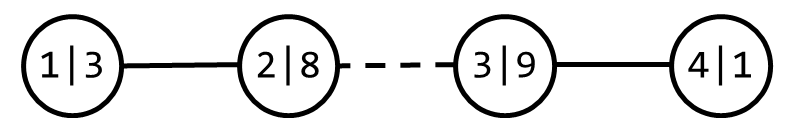
\includegraphics[scale=0.5]{example1.png}

Giải thích cho ví dụ thứ nhất
\end{center}

\begin{center}
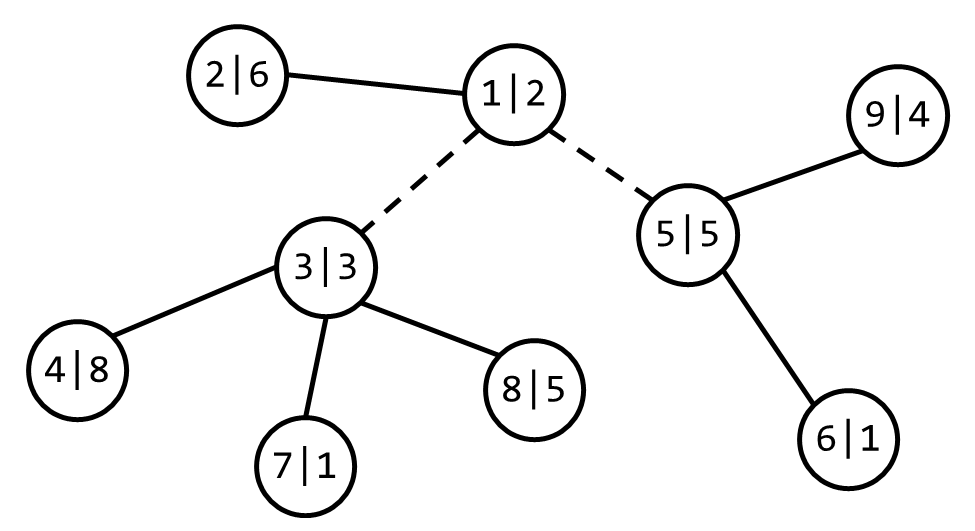
\includegraphics[scale=0.5]{example2.png}

Giải thích cho ví dụ thứ hai
\end{center}
 
\end{problem}